\section{Transformatorn}
\textbf{HAREC a.\ref{HAREC.a.2.4}\label{myHAREC.a.2.4}}
\label{transformatorn}

\subsection{Allmänt}

En transformator består av en eller flera lindningar eller spolar av elektriska
ledare. Lindningarna är magnetiskt kopplade till varandra. Det innebär att de är
anordnade så, att ett magnetfält, som alstrats i någon av lindningarna, även
passerar genom övriga lindningar.

När en växelspänning läggs över en lindning, kallas den primärlindning. I och
omkring primärlindningen alstras då ett magnetiskt fält som växlar i takt med
spänningen. Primärfältet passerar även genom övriga lindningar --
sekundärlindningarna -- och alstrar där spänningar och strömmar.

Den s.k. kopplingsfaktorn mellan lindningarna varierar för olika frekvenser, sämre
vid låga frekvenser (hundratals Hz) och bättre vid höga frekvenser (tusentals
Hz). Speciellt vid låga frekvenser behövs en bättre koppling för att avsedd
effekt ska kunna överföras mellan lindningarna. Då kan ledningsförmågan i den
magnetiska flödesvägen ökas med hjälp av en järnkärna.

\begin{figure}[h]
%  \begin{mdframed}
    \begin{center}
      \begin{circuitikz}
        \draw
        (1,1) node[transformer](T1) {}
        (T1.base) node{1}
        ;
        \draw[european]
        (4,1) node[transformer](T2) {}
        (T2.base) node{2}
        ;
        \draw
        (7,1) node[transformer core](T3) {}
        (T3.base) node{3}
        ;
      \end{circuitikz}
      \\
      \begin{tabular}{ll}
        1, 2 & Allmänna symboler \\
        3 & Transformator med kärna
      \end{tabular}
    \end{center}
    \caption{Schemasymboler för transformatorer}
%  \end{mdframed}
  \label{fig:BildII2-5}
\end{figure}

Bild \ref{fig:BildII2-5} illustrerar flera vanligt förekommande schemasymboler
för transformatorer med två lindningar.

\subsection{Utföranden}

Transformatorn kan utföras för olika ändamål, t.ex. som
\begin{itemize}
\item spänningstransformator,
\item strömtransformator eller
\item impedanstransformator
\end{itemize}
Utförandet påverkas även av överförd effekt
och frekvens.

\subsection{Terminologi}

\begin{tabular}{ll}
primärkrets & sekundärkrets \\
primärlindning & sekundärlindning \\
primärspänning \(u_1\) &  sekundärspänning \(u_2\) \\
primärström \(i_1\) & sekundärström \(i_2\) \\
lindningsvarvtal n & primärt \(n_1\) sekundärt \(n_2\)
\end{tabular}

varvtalsomsättning = \(\dfrac{n_1}{n_2}\) eller \(\dfrac{n_2}{n_1}\)

impedansomsättning = \(\dfrac{Z_1}{Z_2}\) eller \(\dfrac{Z_2}{Z_1}\)

\subsection{Den ideala (förlustfria) transformatorn}
\textbf{HAREC a.\ref{HAREC.a.2.4.1}, a.\ref{HAREC.a.2.4.2.1},
a.\ref{HAREC.a.2.4.2.2}\label{myHAREC.a.2.4.1}
\label{myHAREC.a.2.4.2.1}\label{myHAREC.a.2.4.2.2}}

\emph{Transformering av spänning och ström}

Transformatorn är obelastad när sekundärkretsen är bruten.

\begin{figure*}[h]
\begin{center}
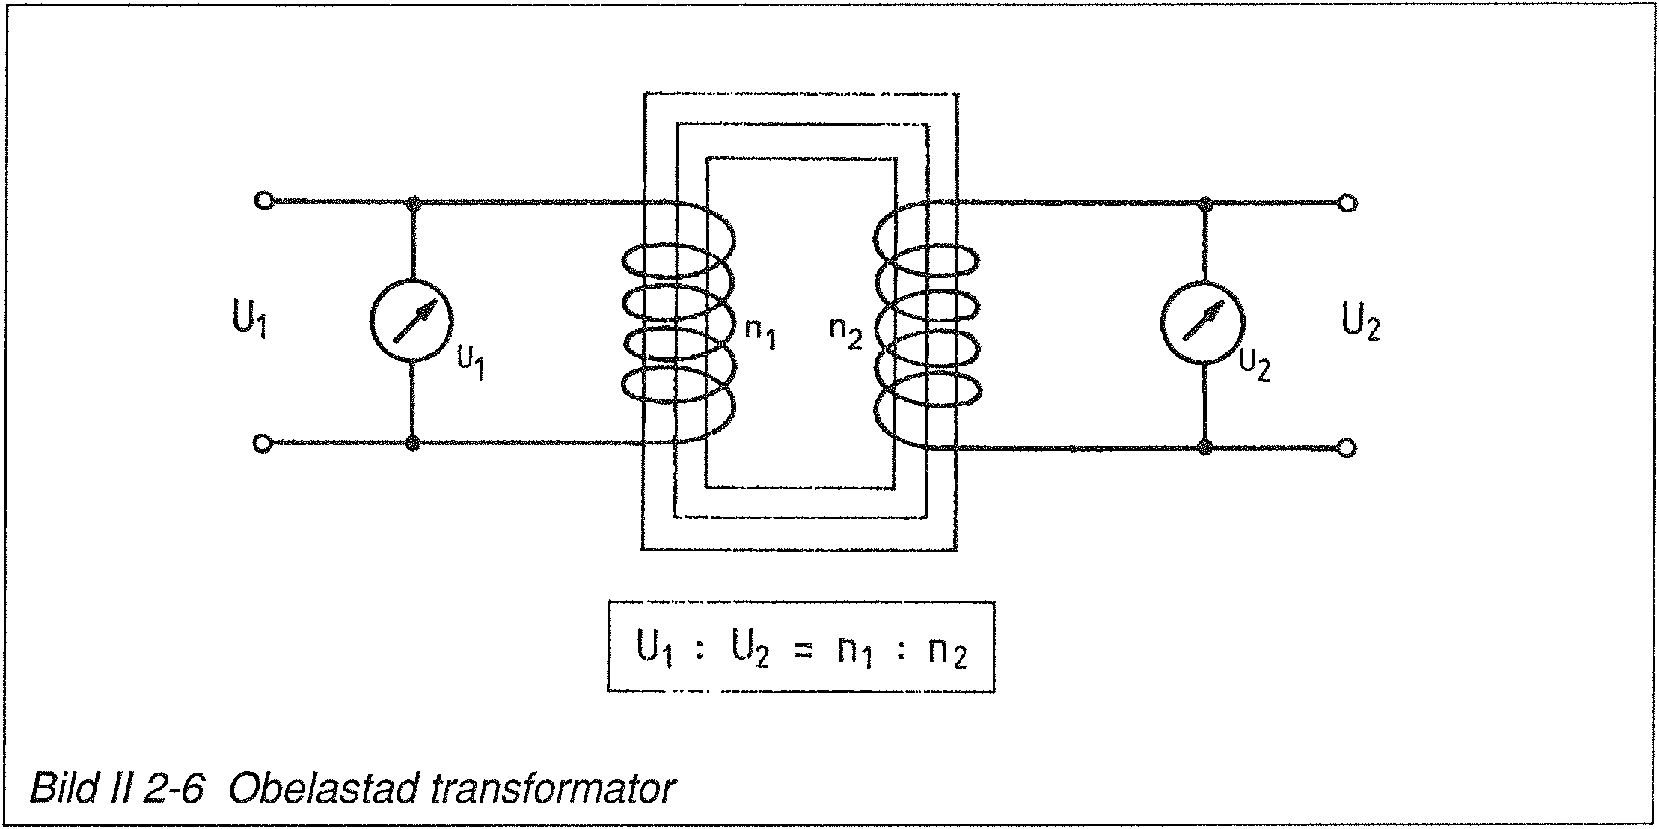
\includegraphics[width=\textwidth]{images/bild_2_2-06}
\caption{Obelastad transformator}
\label{fig:BildII2-6}
\end{center}
\end{figure*}

Bild \ref{fig:BildII2-6}

När primärlindningen ansluts till en växelspänning, induceras det
växelspänningar både över primär- och sekundärlindningarna. Det uppstår även en
ström i primärlindningen, men däremot inte i sekundärlindningen när
sekundärkretsen är bruten. För den obelastade transformatorn gäller sambandet

\(\dfrac{u_1}{u_2} = \dfrac{n_1}{n_2}\)

d.v.s. spänningen över lindningarna är proportionell med lindningsvarvtalet.

Transformatorn är belastad när sekundärkretsen är sluten.

\begin{figure*}[h]
\begin{center}
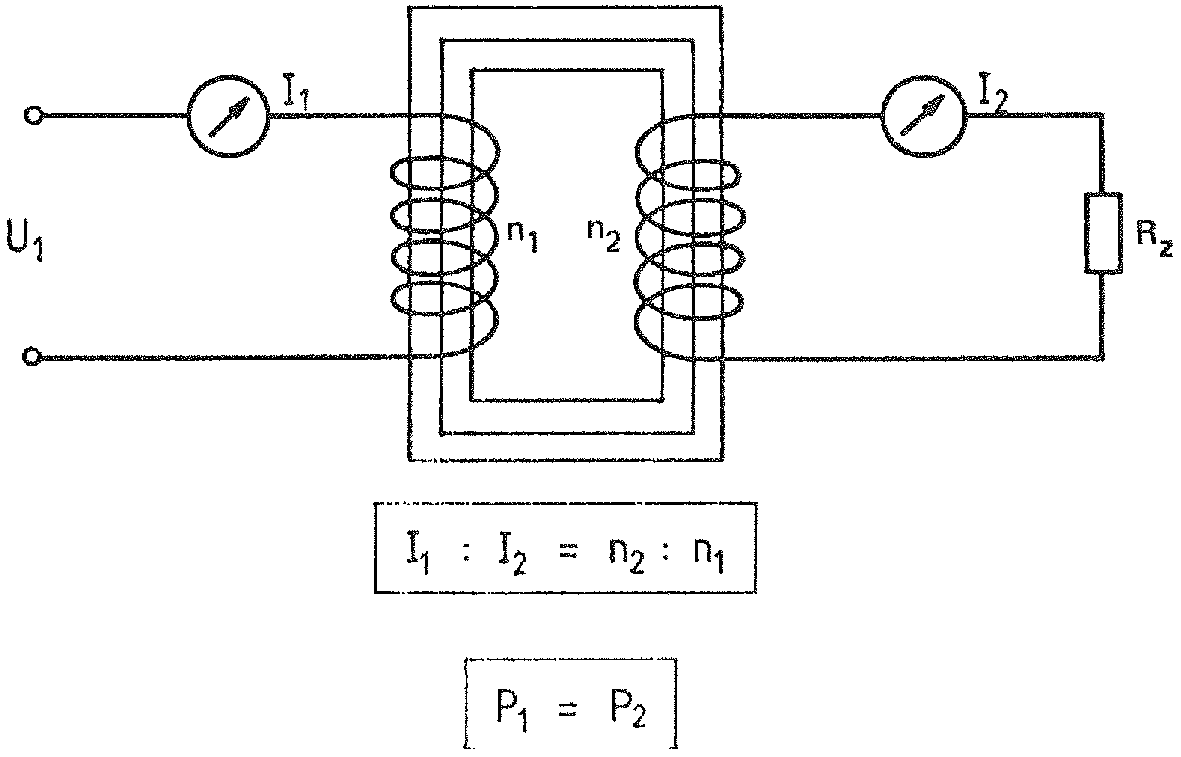
\includegraphics[width=\textwidth]{images/bild_2_2-07}
\caption{Belastad transformator}
\label{fig:BildII2-7}
\end{center}
\end{figure*}

Bild \ref{fig:BildII2-7}

När någon av transformatorns sekundärlindningar ingår i en sluten strömkrets,
uppstår en sekundärström där.

Sekundärströmmen alstrar ett magnetfält, som motverkar primärströmmens fält,
hindrar dess växlingar och tar ut energi från primärkretsen.

Strömförbrukningen på primärsidan ökar således i proportion till
strömförbrukningen på sekundärsidan. Transformatorn reglerar själv hur mycket
energi som den tar från strömkällan och lagrar i fältet för att föra över
till sekundärkretsen.

För den belastade transformatorn gäller, att strömmen genom lindningarna är
omvänt proportionell med lindningsvarvtalet.

\(\dfrac{i_1}{i_2} = \dfrac{n_2}{n_1}\)

Av föregående formler följer att:

\(\dfrac{u_1}{u_2} = \dfrac{i_2}{i_1}\)

Av \(P_1 = u_1 \cdot i_1\) och \(P_2 = u_2 \cdot i_2\) följer att \(P_1 = P_2\).

Om man bortser från förlusterna i transformatorn, så är den effekt som den tar
från kraftkällan lika med den effekt den avger.

\subsection{Transformatortillämpningar}
\textbf{HAREC a.\ref{HAREC.a.2.4.2.4}\label{myHAREC.a.2.4.2.4}}

\emph{Sparkopplade transformatorer}

\begin{figure*}[h]
\begin{center}
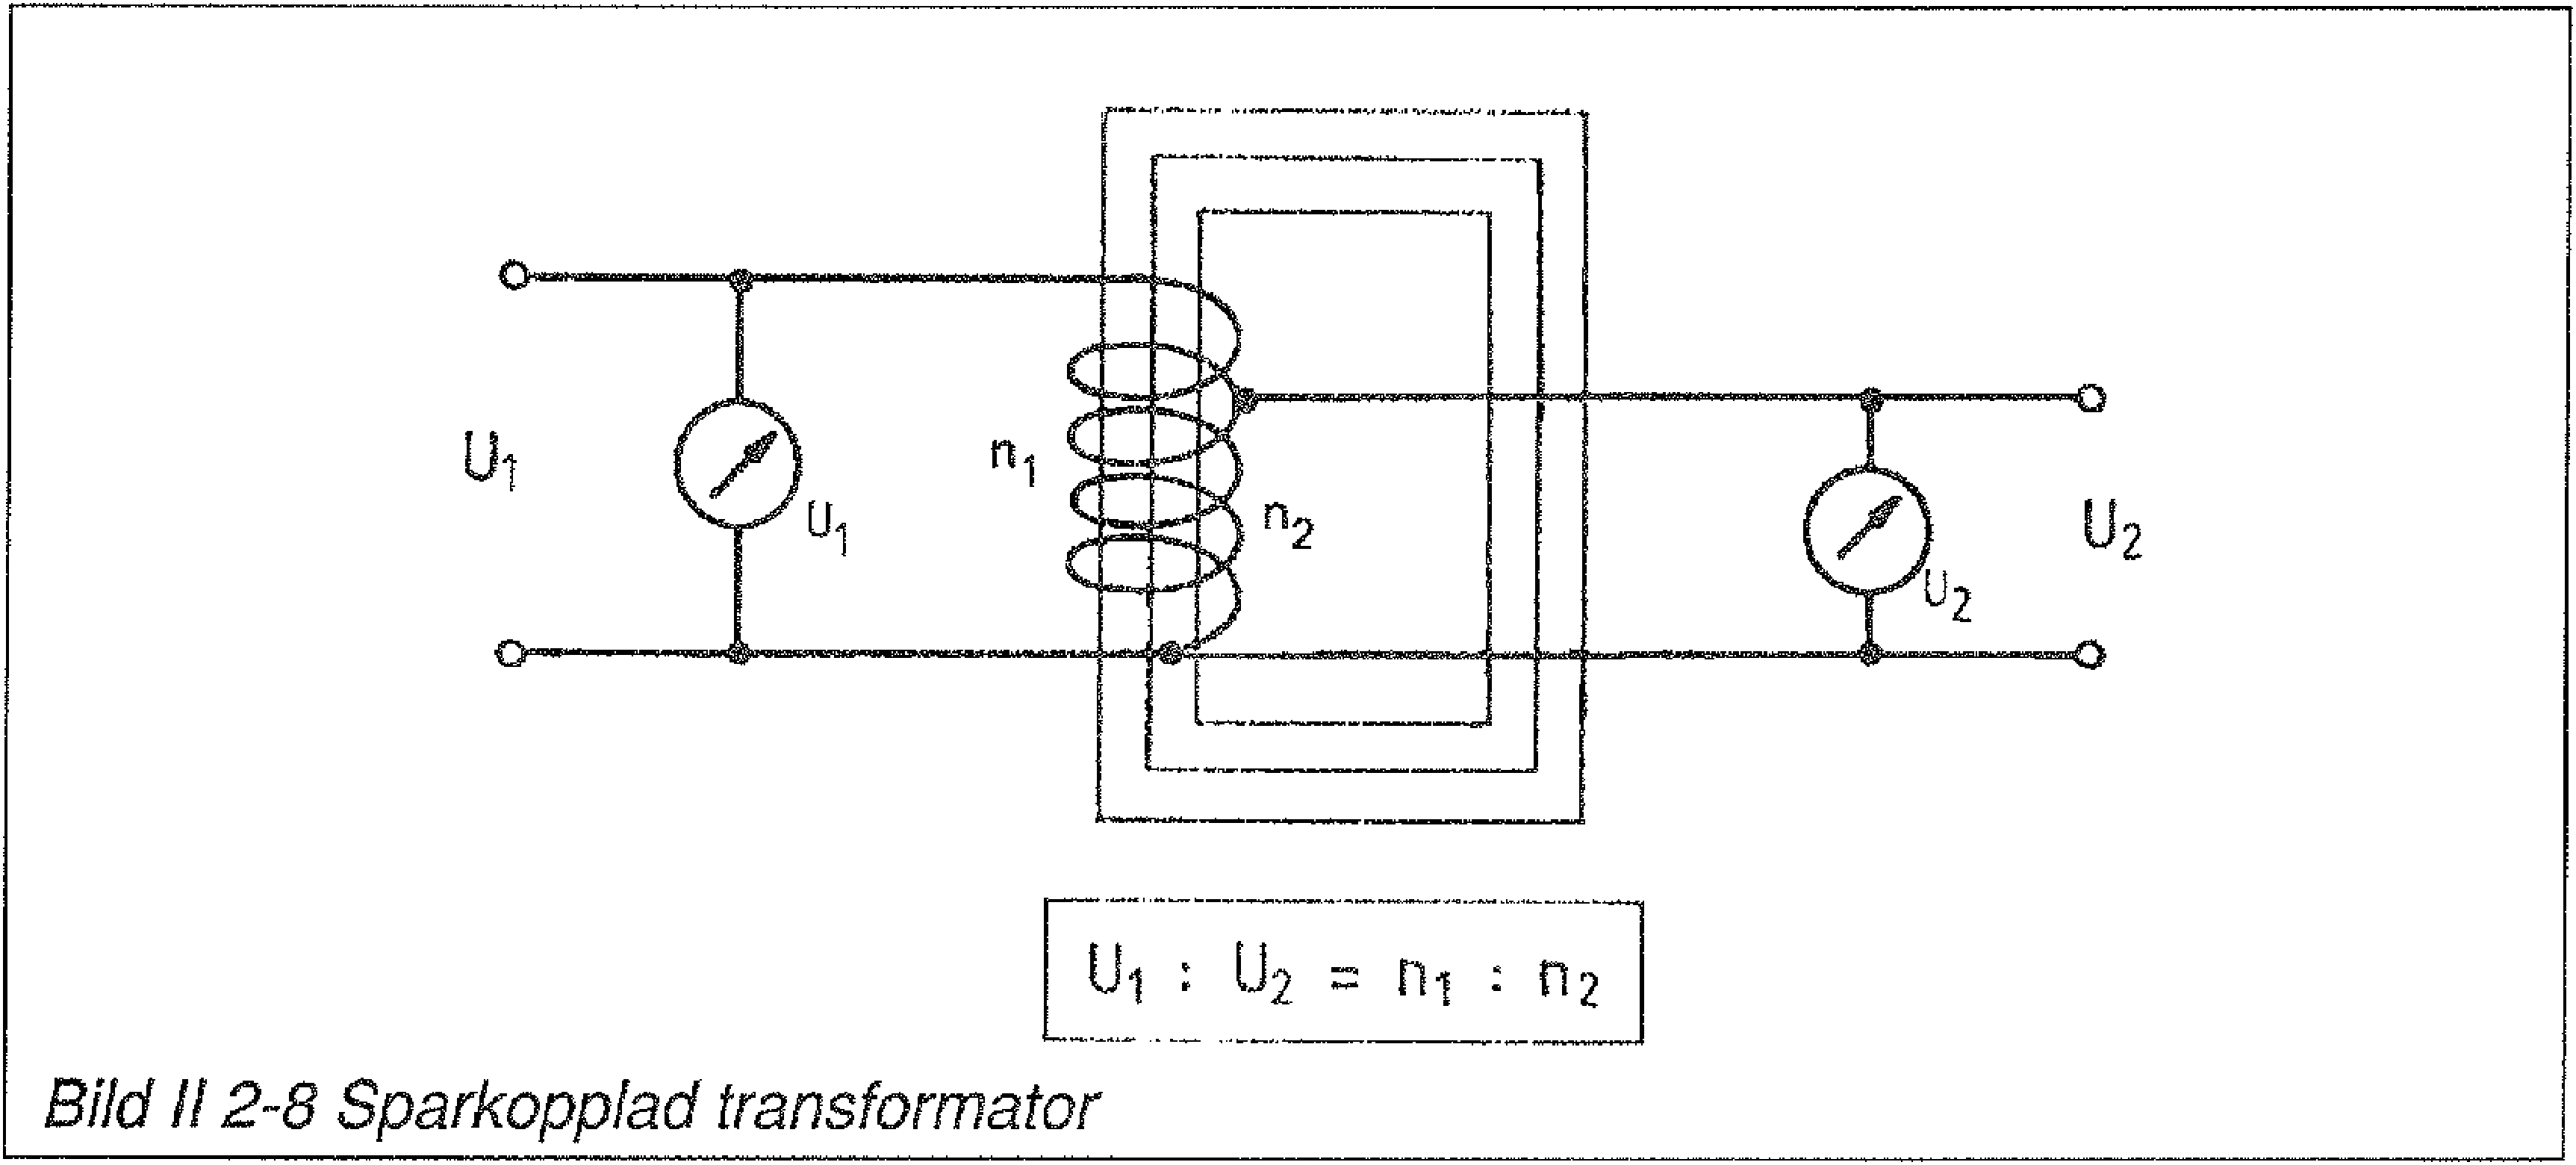
\includegraphics[width=\textwidth]{images/bild_2_2-08}
\caption{Sparkopplad transformator}
\label{fig:BildII2-8}
\end{center}
\end{figure*}

Bild \ref{fig:BildII2-8}

Här ovan har transformatorn beskrivits så att primär- och sekundärlindningarnas
enda förbindelse med varandra är över ett magnetfält, alltså utan galvanisk
förbindelse.

Varje lindning kan emellertid förses med godtyckliga uttag. Över av finns då en
spänning i proportion till det lindningsvarvtal som finns mellan uttagen.

Detta är en metod att spara in på antalet lindningar. För att t.ex. omsätta
nätspänningen 230~V till 115~V används ibland en spartransformator.

Med en spartransformator kommer olika strömkretsar i galvanisk förbindelse med
varandra och särskild försiktighet ska därför iakttas vid användning av
sparkopplade transformatorer, p.g.a. risken för elolycksfall.
Spartransformatorer bör därför inte användas i amatörradiosammanhang. Säkrast
är transformatorer med galvaniskt skilda ledningar och dessutom med speciellt
bra isolering och kapsling -- s.k. skyddstransformatorer.

\emph{Strömtransformatorer}

Hög sekundärström under låg sekundärspänning kännetecknar en strömtransformator.
Strömtransformatorer används i elektriska svetsningsutrustningar,
induktionsugnar o.s.v. Strömtransformatorer används även för mätning av höga
växelströmmar.

\begin{figure*}[h]
\begin{center}
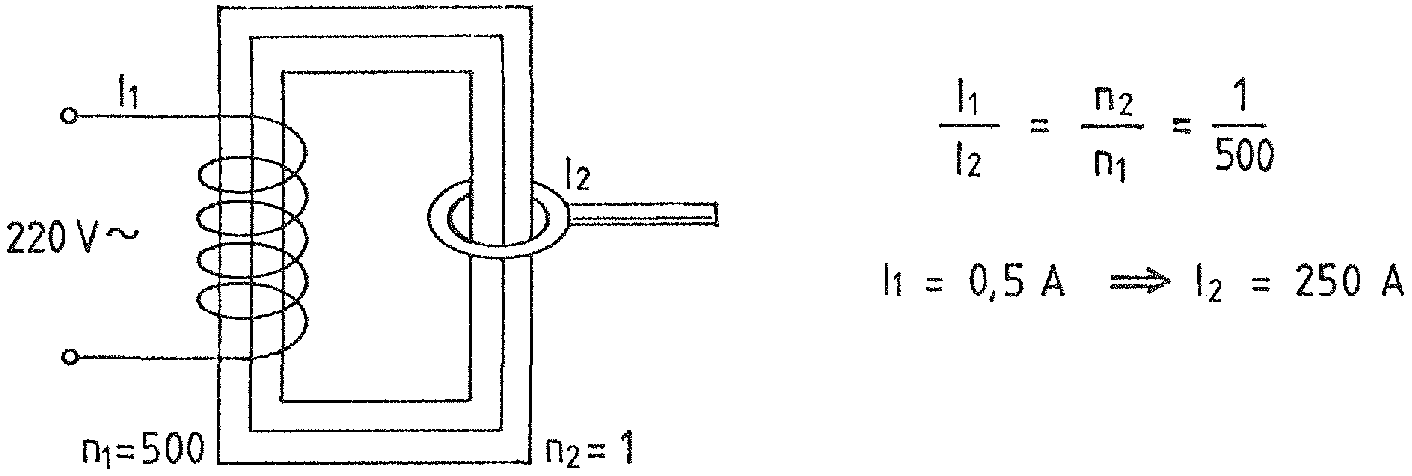
\includegraphics[width=\textwidth]{images/bild_2_2-09}
\caption{Strömtransformator}
\label{fig:BildII2-9}
\end{center}
\end{figure*}

Bild \ref{fig:BildII2-9}

\emph{Högspänningstransformatorer}

Hög sekundärspänning under förhållandevis låg sekundärström kännetecknar en
spänningstransformator.

Högspänningstransformatorer används i distributionsnät, neonskyltar, tändsystem
för förbränningsmotorer, anodspänningsaggregat för sändare o.s.v.

\begin{figure*}[h]
\begin{center}
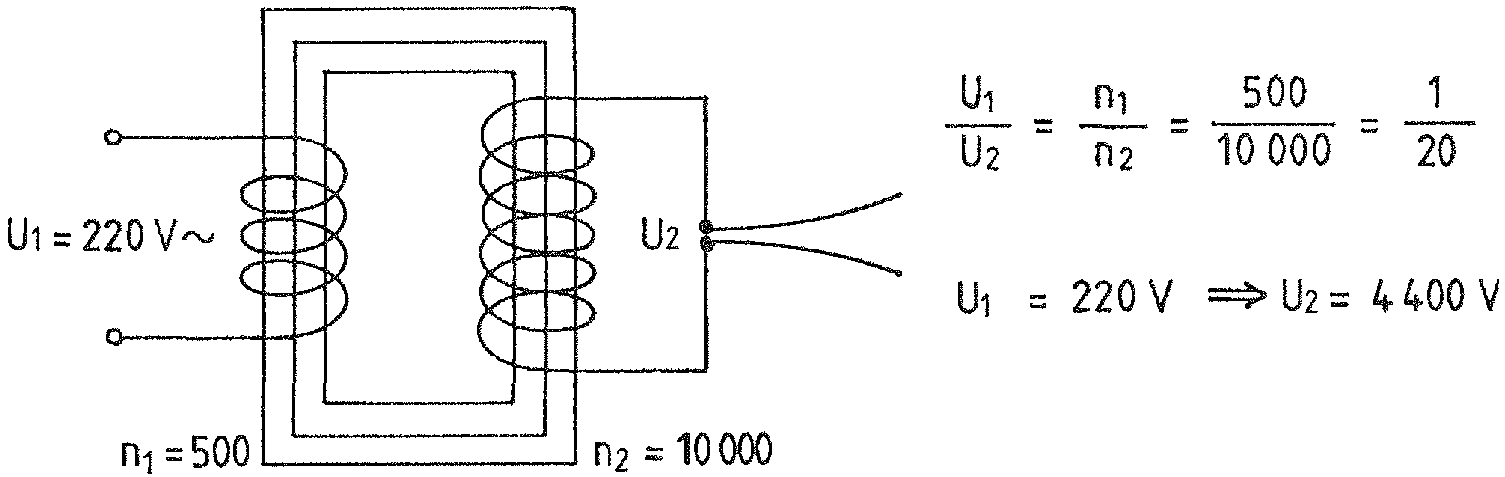
\includegraphics[width=\textwidth]{images/bild_2_2-10}
\caption{Högspänningstransformator}
\label{fig:BildII2-10}
\end{center}
\end{figure*}

Bild \ref{fig:BildII2-10}

Bilden visar en transformator med ett gnistgap i sekundärkretsen för tändning av
gas.

\emph{Låg- och klenspänningstransformatorer}

\begin{figure*}[h]
\begin{center}
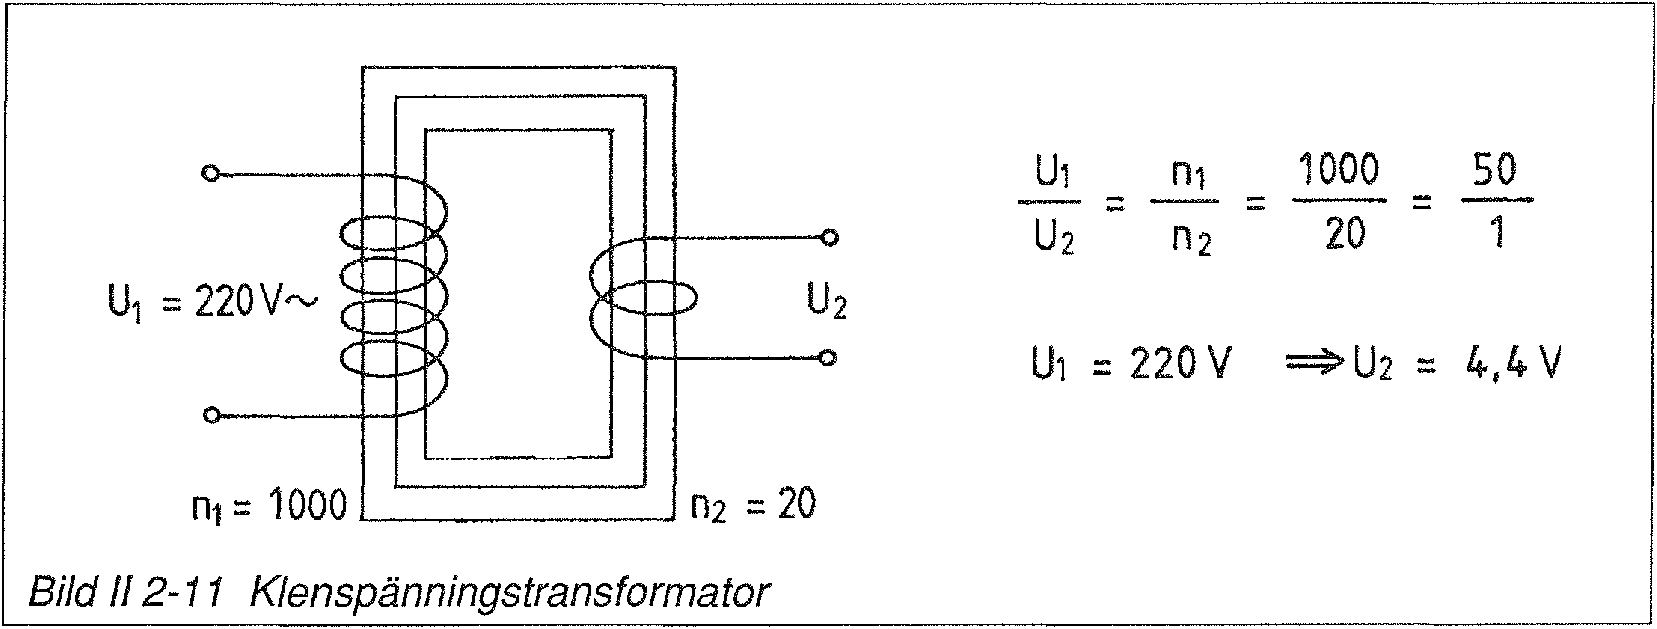
\includegraphics[width=\textwidth]{images/bild_2_2-11}
\caption{Klenspänningstransformator}
\label{fig:BildII2-11}
\end{center}
\end{figure*}

Bild \ref{fig:BildII2-11}

Lågspänningstransformatorer används i lokala distributionsnät, vanligen med
spänningen 400/230~V. För ökad säkerhet mot elektrisk chock krävs dock att vissa
apparater drivs med en s.k. klenspänning av högst 50~V över en s.k.
skyddstransformator med förstärkt isolering.

\subsection{Sambandet mellan varvtal och impedans}
\textbf{HAREC a.\ref{HAREC.a.2.4.2.3}\label{myHAREC.a.2.4.2.3}}
\index{impedans!transformator varvtal}

Transformatorn kan även användas för anpassning av impedanser. Impedansen Z i en
lindning är proportionell mot kvadraten av dess lindningsvarvtal n.

Om effekten i sekundärlindningen är lika stor som i primärlindningen, gäller
formeln

\(\dfrac{Z_p}{Z_s} = \dfrac{n_p^2}{n_s^2}\)
